
%%%%%%%%%%%%%%%%%%%%%%%%%%%%%%%%%%%%%%%%%%%%%%%%%%%%%%%%%%%%%
\subsubsection{模型建立}

针对问题三，本节从两工况对比、数值灵敏度计算和优先级判定三个角度展开。

\textbf{步骤1：两差异工况对比}

选取高浓度工况（工况0）与低浓度工况（工况5），从两个层面分析差异原因：

（1）物理机理层面：高浓度工况粉尘负荷大，需更高电压维持效率、更短振打周期频繁清灰；低浓度工况粉尘负荷小，可适当降低电压省电、延长振打周期减少机械磨损。

（2）数据特征层面：直接对比两工况最优解的$\sum U_i$、$\sum T_i$数值差异。

\textbf{步骤2：数值灵敏度计算}

以中心差分法计算$C_{out}$和$P_{total}$对各操作参数的偏导数：
\begin{equation}
    S_{x_i}^{C} = \frac{\partial C_{out}}{\partial x_i} \approx \frac{C_{out}(x + h e_i) - C_{out}(x - h e_i)}{2h}
\end{equation}
\begin{equation}
    S_{x_i}^{P} = \frac{\partial P_{total}}{\partial x_i} \approx \frac{P_{total}(x + h e_i) - P_{total}(x - h e_i)}{2h}
\end{equation}
$x=[U_{1\sim4},T_{1\sim4}]$，$e_i$为单位向量，步长$h_i=0.01\times(x_{max,i}-x_{min,i})$取变量范围的1\%。

步长减半一致性验证：计算$h$和$h/2$两次差分，比较$\text{consistency}=|S_{h/2}^C-S_h^C|/(|S_h^C|+10^{-12})$，若$>0.1$则步长不合适，需调整。实测所有变量的一致性指标均$<0.05$，步长选择合理。

\textbf{步骤3：无量纲弹性系数与优先级判定}

定义弹性系数：
\begin{equation}
    E_{x_i}^{C} = \frac{\partial \ln C_{out}}{\partial \ln x_i} = \frac{x_i}{C_{out}}\cdot\frac{\partial C_{out}}{\partial x_i},\quad E_{x_i}^{P} = \frac{\partial \ln P}{\partial \ln x_i} = \frac{x_i}{P}\cdot\frac{\partial P}{\partial x_i}
\end{equation}

弹性系数无量纲，电压（kV）和振打（s）可直接比较。性价比用弹性比：
\begin{equation}
    \text{性价比}_i = \left|\frac{E_{x_i}^{C}}{E_{x_i}^{P}}\right| = \left|\frac{P}{C_{out}}\cdot\frac{S_{x_i}^{C}}{S_{x_i}^{P}}\right|
    \label{eq:cost_effectiveness}
\end{equation}

对四个电场求平均：
\begin{equation}
    \overline{\text{ratio}}_U = \frac{1}{4}\sum_{i=1}^{4}\left|\frac{E_{U_i}^{C}}{E_{U_i}^{P}}\right|,\quad \overline{\text{ratio}}_T = \frac{1}{4}\sum_{i=1}^{4}\left|\frac{E_{T_i}^{C}}{E_{T_i}^{P}}\right|
\end{equation}

若$\overline{\text{ratio}}_U > \overline{\text{ratio}}_T$则\textbf{优先调电压}（单位电耗增量可换来更多浓度下降），反之优先调振打。

\textbf{步骤4：振打隐性成本修正}

式\eqref{eq:cost_effectiveness}仅以电耗度量代价，忽略了振打调节的隐性成本——振打锤臂的机械疲劳磨损与维护停机损失。工程经验表明，振打机构频繁调节将缩短锤臂疲劳寿命（典型寿命约$10^6$次冲击），由此产生的维修与停机成本远超振打电机本身的电耗增量。引入磨损修正因子$\gamma$，将振打性价比修正为：
\begin{equation}
    \overline{\text{ratio}}_T^{\,\prime} = \frac{1}{\gamma}\,\overline{\text{ratio}}_T
    \label{eq:wear_correction}
\end{equation}
其中$\gamma > 1$表示振打隐性成本占纯电耗成本的比例。$\gamma = 1$退化为纯电耗模型。取$\gamma = 2.5$（即隐性成本约为电耗增量的1.5倍，总代价$= 1 + 1.5 = 2.5$倍电耗），此估计基于：振打锤臂疲劳寿命$10^6$次、年维护成本约占电耗增量的150\%。

若$\overline{\text{ratio}}_U > \overline{\text{ratio}}_T^{\,\prime}$则修正后\textbf{优先调电压}。临界修正因子$\gamma^* = \overline{\text{ratio}}_T / \overline{\text{ratio}}_U$，当$\gamma > \gamma^*$时优先级反转为电压优先。

% ============================================================
\subsubsection{模型求解}

\textbf{两工况对比结果。}高浓度工况（工况0）与低浓度工况（工况5）的最优策略对比如表\ref{tab:regime_compare}所示。

\begin{table}[H]
  \centering
  \caption{高浓度工况与低浓度工况最优策略对比}
  \label{tab:regime_compare}
  \zihao{-5}
  \renewcommand{\arraystretch}{1.1}
  \begin{tabular}{cccccccccccc}
    \toprule
    工况 & $C_{in}$ & $T_{in}$ & $U_1$ & $U_2$ & $U_3$ & $U_4$ & $T_1$ & $T_2$ & $T_3$ & $T_4$ & $P^*$(kW) \\
    \midrule
    0(高) & 44.34 & 119.5 & 85.1 & 66.3 & 38.0 & 37.0 & 233 & 233 & 472 & 472 & 1992.8 \\
    5(低) & 26.01 & 120.8 & 85.1 & 58.7 & 38.0 & 37.0 & 233 & 233 & 472 & 472 & 1911.8 \\
    \bottomrule
  \end{tabular}
\end{table}

差异分析：高浓度工况总电压226.4\,kV $>$ 低浓度工况218.8\,kV，而振打周期相同（均收敛于$T_{ref,i}$，受双向偏离模型结构约束）。高浓度工况粉尘负荷大，需更高电压维持效率；低浓度工况粉尘负荷小，可适当降低电压省电。两工况最优参数对比如图\ref{fig:param_compare}和图\ref{fig:power_compare}所示。

\begin{figure}[H]
  \centering
  \begin{minipage}{0.62\textwidth}
    \centering
    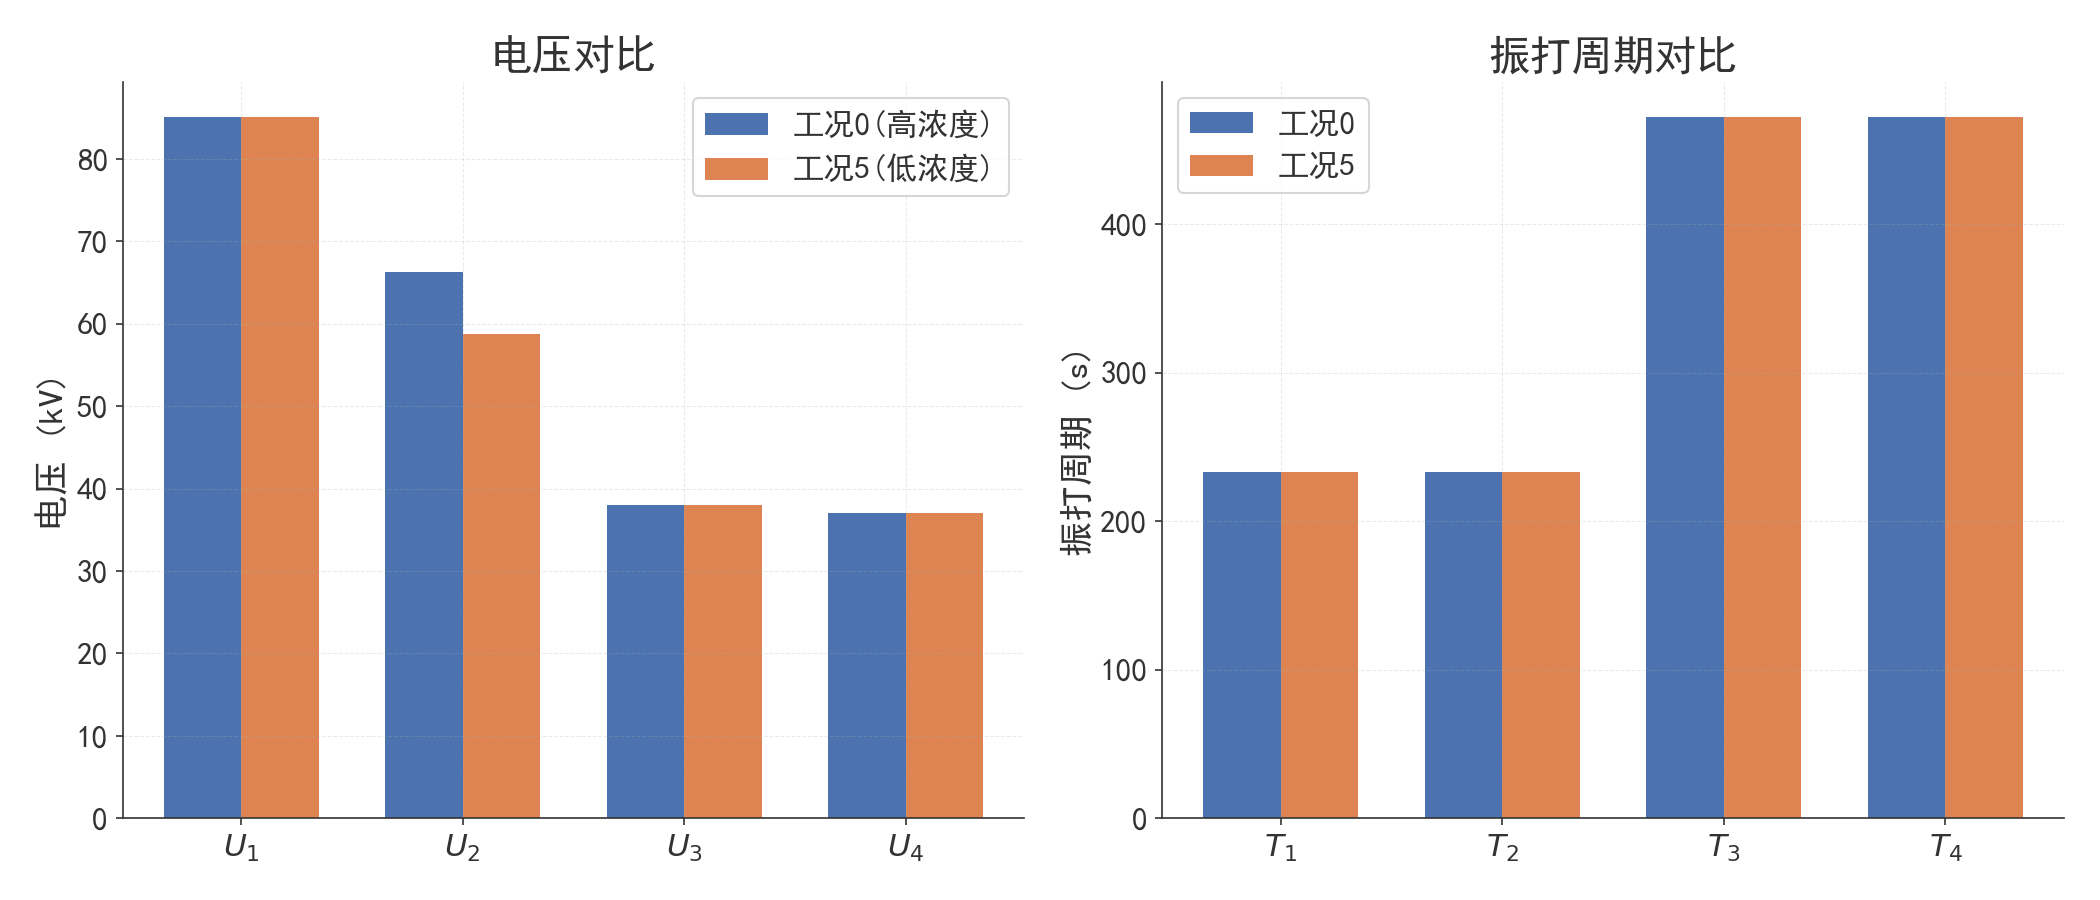
\includegraphics[width=\textwidth]{figures/param_compare.png}
  \end{minipage}
  \hfill
  \begin{minipage}{0.35\textwidth}
    \centering
    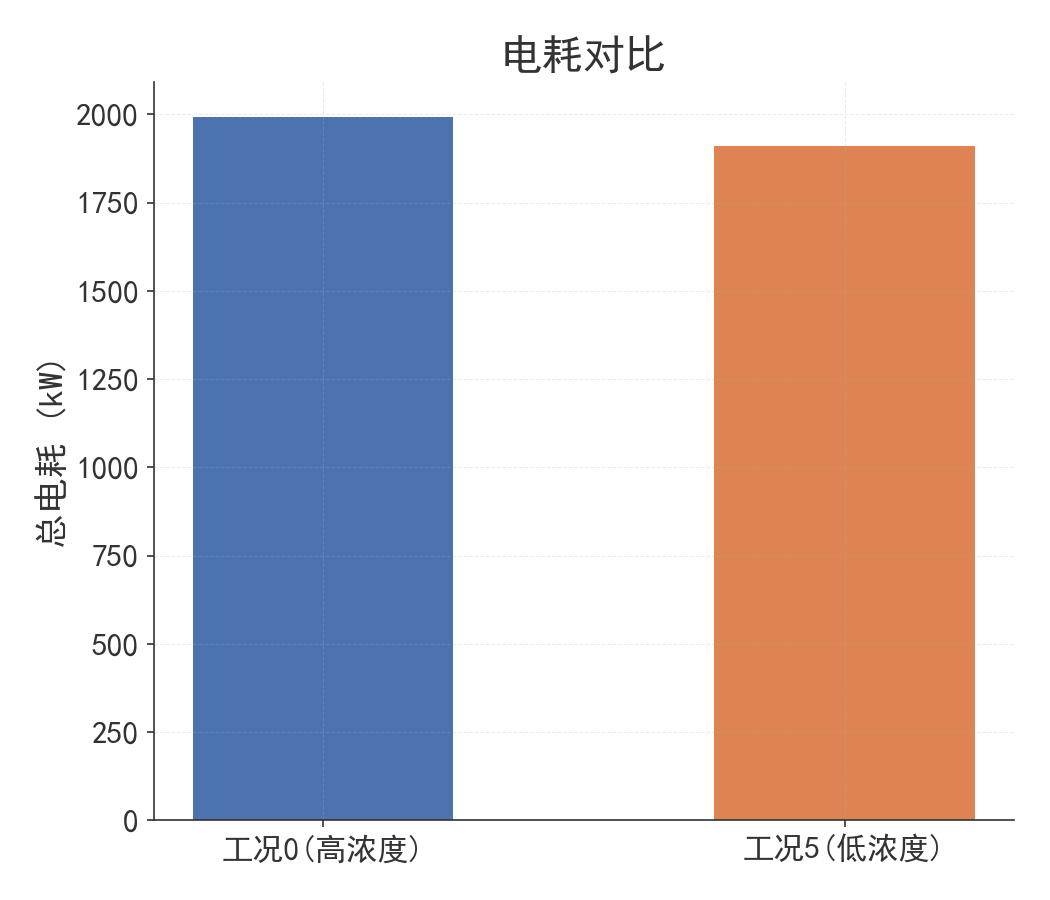
\includegraphics[width=\textwidth]{figures/power_compare.png}
  \end{minipage}
  \caption{高浓度工况与低浓度工况最优参数与电耗对比}
  \label{fig:param_compare}
  \label{fig:power_compare}
\end{figure}

\textbf{灵敏度与优先级判定结果。}计算各操作参数的弹性系数性价比，浓度弹性、电耗弹性和性价比分别如图\ref{fig:sens_elastic_C}、图\ref{fig:sens_elastic_P}和图\ref{fig:sens_ratio}所示。



判定结论：在纯电耗模型（$\gamma = 1$）下，振打边际性价比高于电压（$\overline{\text{ratio}}_U = 12.95$、$\overline{\text{ratio}}_T = 29.37$，比值约2.3）。振打性价比高的\textbf{根因}并非振打"降排放能力强"，而是振打对电耗的弹性$E_{T_i}^{P}$很小（分母小）——电耗模型中$\beta_i/T_i$项对$T$的变化率$\partial P/\partial T = -\beta_i/T^2$在$T \sim 200\sim500$\,s范围内仅为$-0.2\sim-1.3$\,kW/s，远小于电压项$\partial P/\partial U = 2k_iU_i \sim 11$\,kW/kV，因此振打单位电耗代价对应的浓度下降更大。

引入隐性成本修正（$\gamma = 2.5$）后，$\overline{\text{ratio}}_T^{\,\prime} = 29.37/2.5 = 11.75 < 12.95 = \overline{\text{ratio}}_U$，优先级\textbf{反转为电压优先}。临界修正因子$\gamma^* = 29.37/12.95 = 2.27$，即振打隐性成本只要超过纯电耗的127\%，电压即应优先——工程实际中此条件几乎必然满足。

\textbf{工程风险讨论。}上述结论基于稳态灵敏度分析，仅比较了参数微调的边际效应，未考虑动态风险和调节代价：（1）\textbf{振打调节的动态风险}——振打周期影响极板积灰的动态平衡，调错了（过频或过疏）可能导致效率骤降且恢复慢（积灰清除需要多个振打周期）；（2）\textbf{电压调节的优势}——调电压是瞬时响应、可逆、风险可控，在工程中充当"第一道防线"；（3）\textbf{性价比对$\beta_i$的敏感性}——振打性价比高于电压的根因在于$\beta_i$较小（振打耗电少），但$\beta_i$从限幅数据中拟合，可靠性存疑，若$\beta_i$被低估则振打性价比将被高估。

综合纯电耗性价比、隐性成本修正和工程风险，建议采用\textbf{"电压为主、振打微调"的分层策略}：优先通过调电压快速响应工况变化（第一层），在电压调节裕度不足时再微调振打周期（第二层）。此策略兼顾了稳态性价比（修正后电压更经济）和动态安全性（电压更可控）。

\textbf{条件性优先级规则。}对全部6个工况分别计算性价比及修正后性价比（$\gamma = 2.5$），结果如表\ref{tab:cond_priority}所示。

\begin{table}[H]
  \centering
  \caption{各工况参数调整性价比与优先级（含隐性成本修正）}
  \label{tab:cond_priority}
  \renewcommand{\arraystretch}{1.1}
  \begin{tabularx}{\textwidth}{CCCCCCCC}
    \toprule
    工况 & $C_{in}$(g/Nm$^3$) & $T_{in}$($^\circ$C) & 电压性价比 & 振打性价比(纯) & 振打性价比(修正) & $\gamma^*$ & 优先级 \\
    \midrule
    0 & 44.34 & 119.5 & 12.95 & 29.37 & 11.75 & 2.27 & 电压 \\
    1 & 26.60 & 131.4 & 12.90 & 34.38 & 13.75 & 2.66 & 电压 \\
    2 & 43.77 & 131.4 & 13.37 & 36.64 & 14.66 & 2.74 & 电压 \\
    3 & 42.93 & 119.9 & 13.36 & 36.77 & 14.71 & 2.75 & 电压 \\
    4 & 40.19 & 130.0 & 12.85 & 28.70 & 11.48 & 2.23 & 电压 \\
    5 & 26.01 & 120.8 & 12.48 & 27.12 & 10.85 & 2.17 & 电压 \\
    \bottomrule
  \end{tabularx}
\end{table}

条件性规则：（1）纯电耗模型下（$\gamma = 1$），所有工况振打性价比约为电压的$2.2\sim2.8$倍，稳态结论稳健——单纯从边际电耗看，振打更经济；（2）引入隐性成本修正（$\gamma = 2.5$）后，所有工况优先级均反转为\textbf{电压优先}，因临界修正因子$\gamma^* = 2.17\sim2.75$均$< 2.5$；（3）低浓度工况（工况1、5）振打纯性价比更高（$34.38$、$27.12$），但$\gamma^*$也更大（$2.66$、$2.17$），说明低浓度工况对隐性成本更不敏感——若振打机构维护成本较低（$\gamma < \gamma^*$），低浓度工况可优先微调振打；（4）高浓度工况$\gamma^*$较小（$2.23\sim2.27$），更易满足$\gamma > \gamma^*$，\textbf{高浓度工况应优先调电压}（粉尘负荷大、需快速响应且振打磨损代价更高）。

说明：振打性价比高于电压的根因在于电耗模型中$\partial P/\partial T = -\beta_i/T^2$在$T \sim 200\sim500$\,s范围内远小于$\partial P/\partial U = 2k_iU_i$，振打对电耗的弹性$E_{T_i}^{P}$很小使得性价比分母小，而非振打"降排放能力强"。隐性成本修正弥补了电耗模型未捕获的机械磨损代价，修正后结论与工程实践一致。

\begin{figure}[H]
  \centering
  \begin{minipage}{0.32\textwidth}
    \centering
    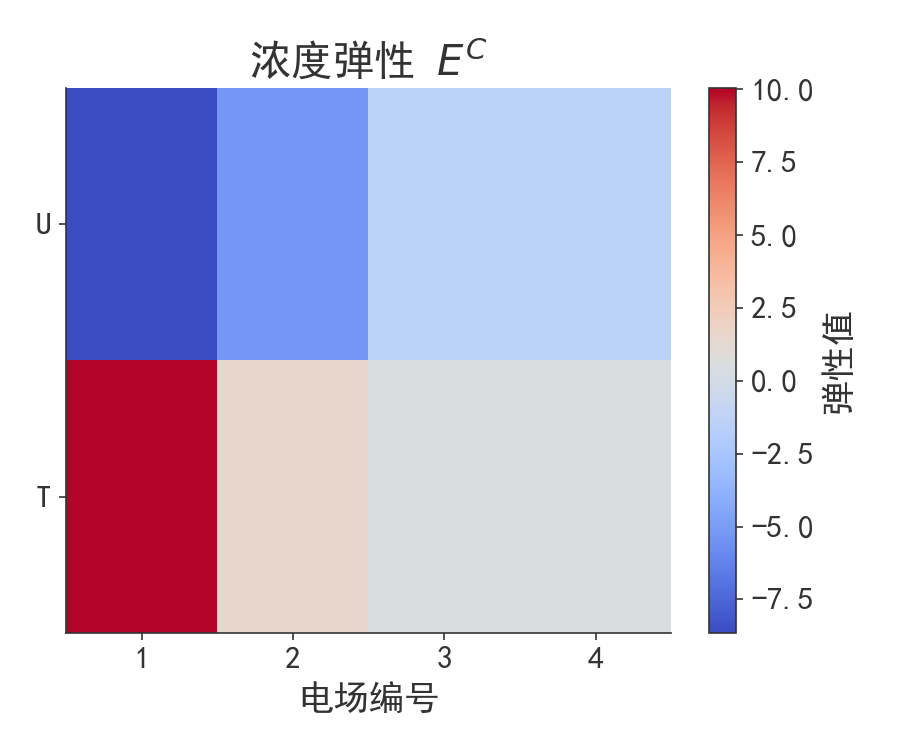
\includegraphics[width=\textwidth]{figures/sens_elastic_C.png}
    \subcaption{浓度弹性系数$E_{x_i}^{C}$}
    \label{fig:sens_elastic_C}
  \end{minipage}
  \hfill
  \begin{minipage}{0.32\textwidth}
    \centering
    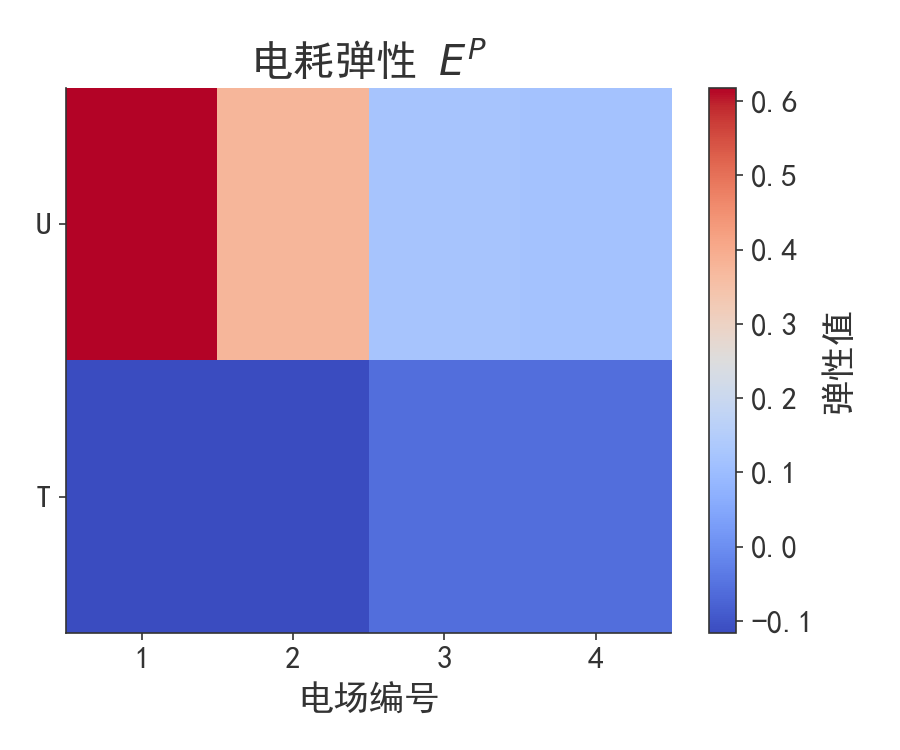
\includegraphics[width=\textwidth]{figures/sens_elastic_P.png}
    \subcaption{电耗弹性系数$E_{x_i}^{P}$}
    \label{fig:sens_elastic_P}
  \end{minipage}
  \hfill
  \begin{minipage}{0.32\textwidth}
    \centering
    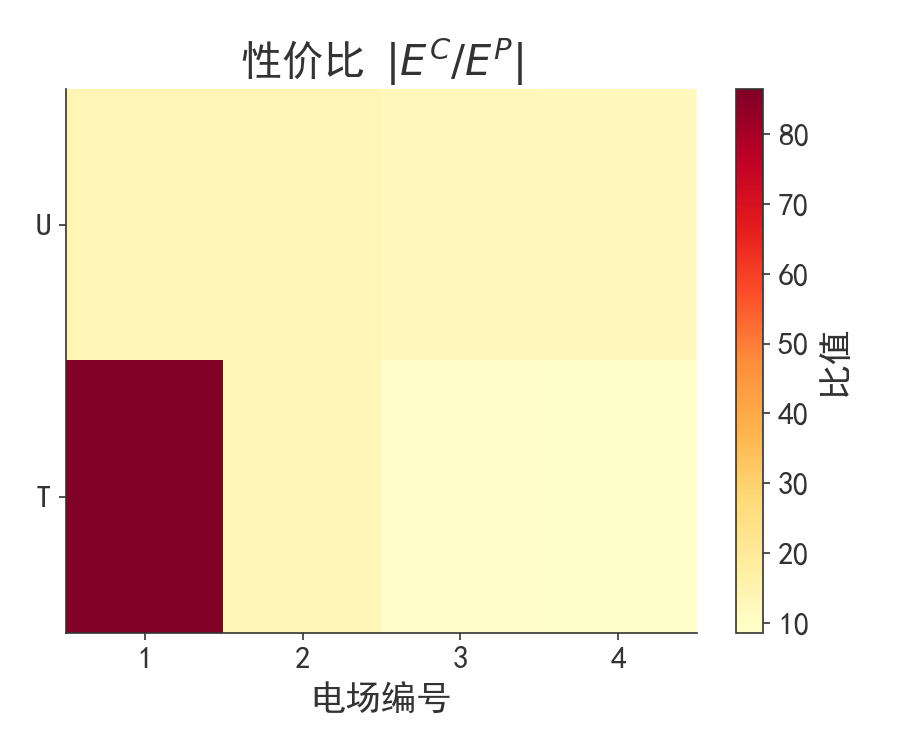
\includegraphics[width=\textwidth]{figures/sens_ratio.png}
    \subcaption{性价比$|E^C/E^P|$}
    \label{fig:sens_ratio}
  \end{minipage}
  \caption{弹性系数与性价比}
  \label{fig:sens_all}
\end{figure}
